\chapter{Steering}
The control of steering wheel take advantage of motor for steering assist originally present in the car. The motor is controlled by a positioning controllers designed for brushed DC and brushless DC motors with encoders. denominated \gls{EPOS} by many manufactures

\section{Maxon EPOS 70/10 controller}
\begin{figure}[h]
	\centering
	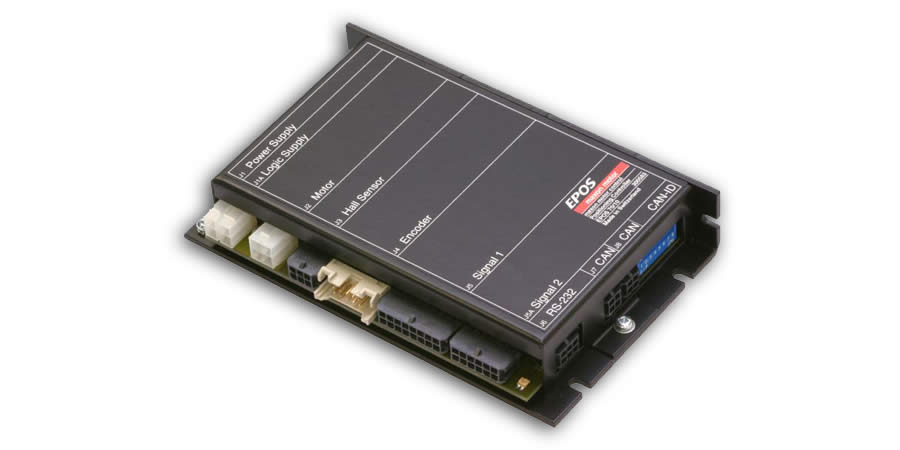
\includegraphics[width=0.5\linewidth]{figures/EPOS-70-10-10-A-11-70VDC-Detail.jpg}
	\caption{Maxon EPOS 70/10 controller}
	\label{fig:maxon_epos}
\end{figure}
The controller available to use is the \href{https://www.maxonmotor.com/maxon/view/product/control/Positionierung/300583}{Maxon EPOS 70/10}, from now on denoted as EPOS. It includes CAN network interface and a RS-232. The relevant electrical specs can be seen in table \ref{tab:epos_specs}. The full specifications as well as connections layout must be seen in \cite{epos_hardware}. The controller contains two led in a single package that is used as status reference. Table \ref{tab:maxon_led_status} present the status of device based on pattern of leds shown by it.

\begin{table}[hb]
	\centering
	\begin{tabular}{lccc}
		\toprule
		\textbf{Description} & \textbf{Min.} & \textbf{Max.} & \textbf{Unity}\\
		\midrule
		Power supply voltage $\text{V}_\text{CC}$ (Ripple \textless 10\%) & 11 & 70 & $\text{V}_\text{DC}$\\
		Max. output voltage & & $0.9\cdot\text{V}_\text{CC}$ & $\text{V}_\text{DC}$\\
		Max. output current $\text{I}_\text{max}$ (\textless 1sec) &  & 25 & A\\
		Continuous output current $\text{I}_\text{cont}$ & & 10 & A\\
		Sample rate PI - current controller &10K & 10K & Hz\\ 
		Sample rate PI - speed controller  &1K & 1K & Hz\\ 
		Sample rate PI - positioning controller &1K & 1K & Hz\\
		Max. speed (motors with 2 poles) & & 25K & rpm\\
		\bottomrule
	\end{tabular}
    \caption{EPOS electric specifications}
    \label{tab:epos_specs}
\end{table}

\begin{table}
	\centering
	\begin{tabular}{p{0.7\textwidth}cc}
		\toprule
		\textbf{Description} & \textbf{Red} & \textbf{Green}\\
		\midrule
		\begin{minipage}{0.4\linewidth}
			The EPOS is in state:
			\begin{itemize}
				\item Switch ON Disabled
				\item Ready to Switch ON
				\item Switched ON
				\item The power stage is disabled
			\end{itemize} 
		\end{minipage} & OFF & Blinking ($\approx$ 1Hz)\\
	    \midrule
	    \begin{minipage}{0.5\linewidth}
	    	The EPOS is in state:
	    	\begin{itemize}
	    		\item Operation Enable
	    		\item Quick Stop Active
	    		\item The power stage is enabled
	    	\end{itemize} 
	    \end{minipage} & OFF & ON\\
        \midrule
        EPOS is in Fault State & ON & OFF\\
        \midrule
        EPOS is in temporary state Fault Reaction Active & ON & ON\\
        \midrule
        There is no valid firmware on the EPOS (due to a failed firmware download) & ON & Flashing \\ 
		\bottomrule
	\end{tabular}
	\caption{Maxon EPOS 70/10 Led status}
	\label{tab:maxon_led_status}
\end{table}


\section{Steering sensor support}
Maxon EPOS 70/10 accepts quadrature sensors to give feedback of position. The used sensor is a quadrature line driver with index (although index is disabled because its track is damaged). The sensor model is HEDR-55L2-BY09 with main characteristics shown in table \ref{tab:quad_sensor} \cite{hedr_sensor}. Table \ref{tab:quad_sensor_settings} show the required configuration to be passed to EPOS device to correctly use the steering controller. See appendix \ref{appendix:maxon} for further description.
\begin{table}[!hb]
	\centering
	\begin{tabular}{lc}
		\toprule
		\textbf{Description} & \textbf{Value}\\
		\midrule
		Line Driver & Yes\\
		Counts per revolution & 3600\\
		Total number of positions & 14400\\
		Shaft diameter & 8mm\\
		\bottomrule
	\end{tabular}
	\caption{Main HEDR-55L2\_BY09 sensor characteristics}
	\label{tab:quad_sensor}
\end{table}

\begin{table}[!hb]
	\centering
	\begin{tabular}{lc}
		\toprule
		\textbf{Description} & \textbf{Value}\\
		\midrule
		Sensor Type & 2\\
		Pulse Number & 3600\\
		Sensor Polarity & 0\\
		\bottomrule
	\end{tabular}
	\caption{Quadrature sensor settings configured in EPOS}
	\label{tab:quad_sensor_settings}
\end{table}

The sensor support is mainly 3D printed in ABS filament. It is composed of the following parts presented in table \ref{tab:sensor_support_parts}.
A dimensional sketch of the sensor and bearing used was also designed just for auxiliary purposes and to provide assembly instructions. The drawings with respective dimensions are added in appendix \ref{appendix:sensor_drawings}. The parts were designed in Autodesk Fusion 360 and are available under the Github repository

\begin{table}[!hb]
    \centering
	\begin{tabular}{lcc}
		\toprule
		\textbf{Part name} & \textbf{Quantity} & \textbf{Reference design}\\
		\midrule
		608 bearing & 1 & \hyperref[draw:bearing]{Bearing Diagram}\\
		Sensor Case HEDR-55L2\_BY09 & 1 & \hyperref[draw:sensor-case]{Sensor case}\\
        Half Gear 54 teeth & 2 & \hyperref[draw:half-gear]{Half gear}\\
        Sensor gear 32 teeth & 1 & \hyperref[draw:sensor-gear]{Sensor gear}\\
		\bottomrule
	\end{tabular}
\caption{Sensor support parts}
\label{tab:sensor_support_parts}
\end{table}



\section{Calibration process}
Here is assumed the vehicle follows a model of Ackermann steering model typical valid for low speed which result in the simplified approximation of the single line model or as in general described in literature, as bicycle model\cite{Snider2009} \cite{Navigation_System_Design}. A simplified representation of the model is present in figure \ref{fig:ackermann_steering}. This model is normally used in control applications and expected to be used in future high level control. As it is necessary to determine the angle of wheel with respect to body frame YY axis (recall subsection \ref{subsection:body_frame}), the first calibration process required is to determine the function relating steering wheel position and angle of fictional wheel. A set up was made fixing the car and placing a white duck tape in front of it, perpendicular as physically possible and apart by 1.47 meters in front of the car. The duck tape will serve as a ruler. In each wheel is attached a laser level, pointing to front duck tape. Several measurements are take for different steering position values and using trigonometric relations, the angles of each wheel is estimated. 
This process will determine the power up offset, minimum and maximum quadrature counter values. These values will only change in case of shut down performed on steering controller device.

\begin{figure}[!hb]
	\centering
	\subcaptionbox{Four wheel representation}{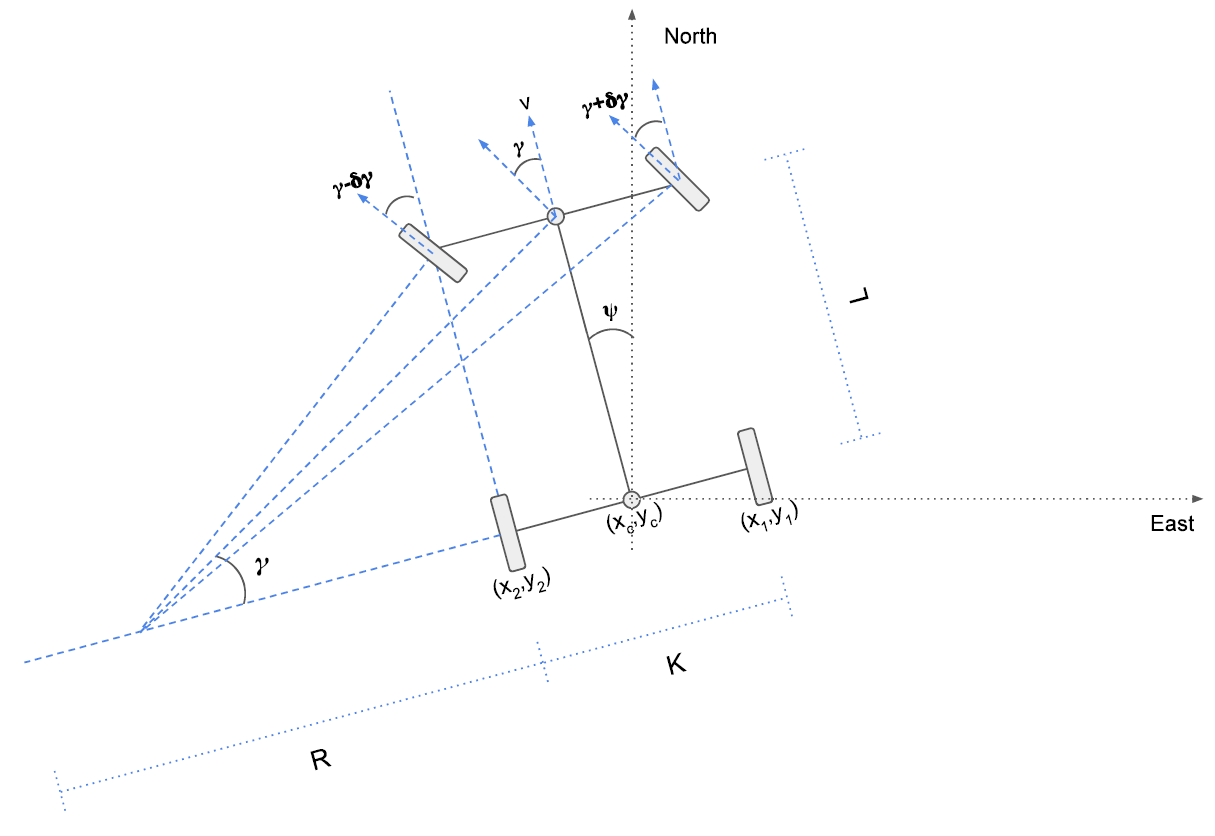
\includegraphics[width=0.7\linewidth]{figures/Ackermann_steering.png}}
	\hfill
	\subcaptionbox{Bicycle Representation (source \cite{Snider2009})}{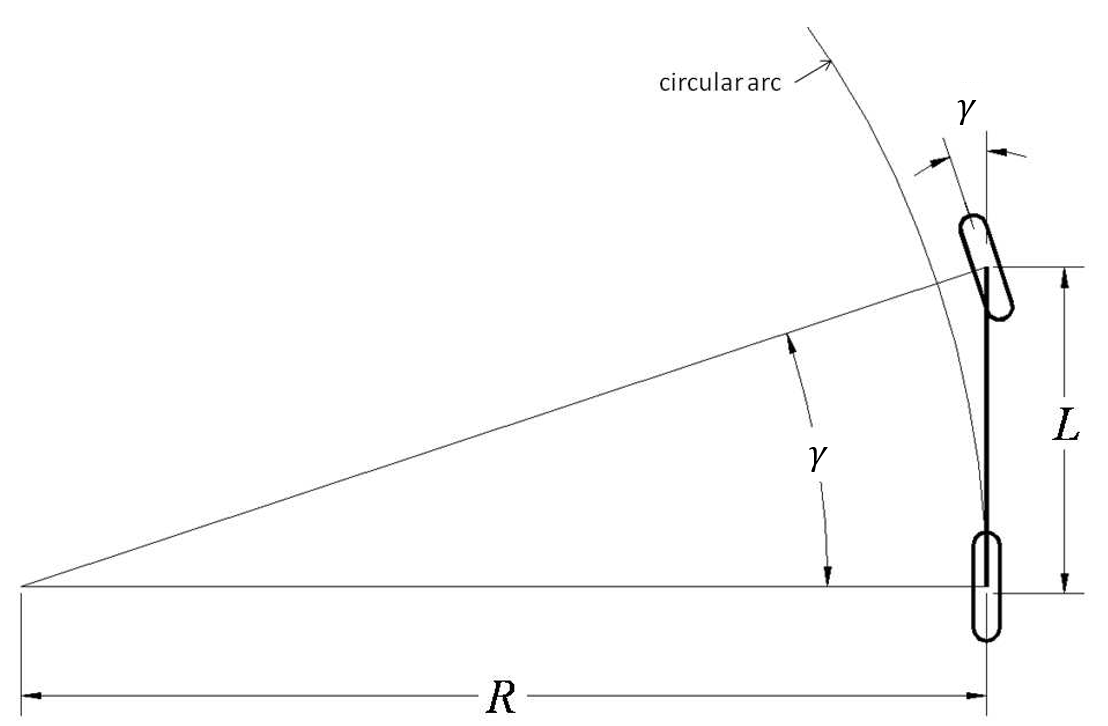
\includegraphics[width=0.5\linewidth]{figures/bicicle_model}}
	\caption{Ackermann steering model simplification}
	\label{fig:ackermann_steering}
\end{figure}

\begin{figure}
	\centering
	\begin{tikzpicture}[scale=2.5]
	\pgfmathsetmacro{\hOne}{1.47};
	\pgfmathsetmacro{\dOne}{1.445};
	\pgfmathsetmacro{\dL}{0.455};
	\pgfmathsetmacro{\maxR}{2.19};
	\pgfmathsetmacro{\maxL}{\maxR};
	\pgfmathsetmacro{\maxRange}{\maxR+\maxL+\dL};
	\pgfmathsetmacro{\lOne}{0.5*(\maxRange-\dL)};
	\pgfmathsetmacro{\lTwo}{0.5*(\dOne-\dL)};
	
	\coordinate (origin) at (0, 0);
	\coordinate (A) at (-\dOne/2, 0);
	\coordinate (B) at (\dOne/2, 0);
	\coordinate (C) at (-\dOne/2, \hOne);
	\coordinate (D) at (\dOne/2, \hOne);
	\coordinate (E) at (-\dOne/2 - \lOne, \hOne);
	\coordinate (F) at (\dOne/2 + \lOne, \hOne);
	\coordinate (zeroR) at (-\dL/2,\hOne);
	\coordinate (zeroL) at (+\dL/2,\hOne);
	
	
	\draw [Bar-Bar , ultra thick] (A)--(0,0) -- (B) node[align=center, below] at (origin) {$d1$};
	\draw [dashed] (A) -- (C) node[below, midway, rotate=90] {$h_1$};
	\draw [dashed] (B) -- (D);
	\draw [dashed] (origin) -- ++(0, 6mm);
	\draw [Bar-Bar,ultra thick] (E)--(F);
	% add angles swipes lines
	\draw [dashed] (A)--(E);
	\draw [dashed] (A)--(zeroL);
	\draw [dashed] (B)--(F);
	\draw [dashed] (B)--(zeroR);
	
	% add zeroR and zeroL nodes
	\node[mark=square, fill, label=above:$0_R$] at (zeroR) {};
	\node[mark=square, fill, label=above:$0_L$] at (zeroL) {};
	% add maxR and maxL nodes
	\node[label=above:$max_R$] at (F) {};
	\node[label=above:$max_L$] at (E) {};
	
	% add arcs of angles
	\filldraw[fill=green!20,draw=green!50!black, dashed] (0,0) -- (0mm,5mm) arc (90:45+90:5mm) node[midway, above]{$\gamma$}-- (0,0);
	
	\filldraw[fill=cyan!20,draw=cyan!50!black, dashed] (A)--($(A)+(0mm,5mm)$) arc (90:56+90:5mm) node[midway, above]{$\beta$} -- (A);
	
	\filldraw[fill=red!20,draw=red!50!black, dashed] (B)--($(B)+(0mm,5mm)$) arc (90:33+90:5mm) node[midway, above]{$\alpha$}--(B);
	
	% add anotations
	\draw [Bar-Bar] (-\dOne/2,\hOne+0.3) -- (-\dL/2,\hOne+0.3) node[align=center, above, midway] {$L_2$};
	\draw [Bar-Bar] (-\dL/2,\hOne+0.3) -- (\dL/2,\hOne+0.3) node[align=center, above, midway] {$d_L$};
	\draw [Bar-Bar] (+\dL/2,\hOne+0.3) -- (\dOne/2,\hOne+0.3) node[align=center, above, midway] {$L_2$};
	\draw [Bar-Bar] (\dOne/2,\hOne+0.3) -- (\dOne/2 + \lOne, \hOne+0.3) node[align=center, above, midway] {$L_1$};
	\draw [Bar-Bar] (-\dOne/2,\hOne+0.3) -- (-\dOne/2 - \lOne, \hOne+0.3) node[align=center, above, midway] {$L_1$};
	\end{tikzpicture}
	\caption{Calibration set up scheme}
	\label{fig:calibration_scheme}
\end{figure}

\section{interface library}
\blindtext